%% future_work.tex
Deep learning is far from being a system with human-like intelligence. Consequently, there is a massive amount of work to be done in the future to get closer to this ultimate goal (while the goal should still be to build a system that supports humans and not behaves like one). However, the implementations presented in this thesis are far from such a system. Consequently, a conclusion is drawn, and the next steps are proposed for the models presented in this thesis, but a long-term vision is presented as well. Specifically, some insights are given to the neuroscientific concept that seems very promising in section \secref{future_neuro_concepts}, and future work is described for horizontal self-organisation in \secref{future_hso} as well as for vertical self-organisation in \secref{future_vso}. Afterwards, in \secref{future_3_stage}, a new model is presented on a very abstract level, which could work better intuitively, but a concrete implementation is unclear. In \secref{useful_representations}, the usefulness of representations is discussed. In the last \secref{cognition_reasoning}, the author gives a personal opinion about the future of AI, which is not supported by scientific arguments but might be interesting for (motivated) readers.



\section{Neuroscientific Concepts}\seclbl{future_neuro_concepts}
In \chref{neuro_concepts}, several concepts from neuroscience are identified that are believed to be fundamental for biological intelligence. However, since the discrepancy between biological and artificial models is large, it is difficult to incorporate these biological concepts into a computer system. This thesis makes concrete suggestions on how such concepts can be implemented. Implementing these concepts in the form of horizontal and vertical self-organisation demonstrates that these ideas can facilitate the learning process. The evaluation of the suitability of neuroscientific concepts was very iterative: many concepts were tested but discarded in the course of the work because they did not add enough value to existing systems. For example, much time was spent on sparsifying activations over several time steps as it is done in the human brain. However, it was found that the sparsification of representations over several time steps has no advantage without additional system dynamics. This could be because the data is static and already contains all the information. Therefore, the result is the same if the sparsification is done in one time step.

The most promising concepts identified in this work for improving deep learning systems are self-organisation, net fragments, sparsity\sidenote{but not over time}, lateral connections, continuous input, and embodiment. For each of these mechanisms, a concept for implementation is proposed, except for continuous input and embodiment. However, these proposals are the author's interpretation and are only one of many possible solutions. These concepts can also be interpreted differently, and an alternative implementation could also lead to promising results. Furthermore, exploring continuous input and embodiment in future work could help to build more intelligent systems. 


\section{Implemented Models}\seclbl{future_so}
The concepts from neuroscience are implemented with two model based on horizontal and vertical self-organisation. It is important to note that the implementation of \emph{neuroscientific concepts} is the main focus of this thesis and not to push scores like accuracy on benchmarks. In general, a comparison with end-to-end backpropagation of error is not appropriate in this field: Backpropagation has been optimised for over 30 years by many institutes and even more researchers, and therefore alternative learning concepts cannot be expected to outperform backpropagation of error instantly. Thus, backpropagation of error is not considered an appropriate baseline.

Rather, the proposed implementations showcase interesting neuroscientific concepts. However, the implementation has not yet been optimised and incorporated in big networks that might perform on the level of existing systems. Rather, these implementations are to be understood as a basis for future work (c.f. \secref{future_3_stage}, \secref*{useful_representations} and \secref*{cognition_reasoning}) that improves AI in the long-term.


\subsection{Horizontal Self-Organisation}\seclbl{future_hso}
The proposed horizontal self-organisation model incorporates neuroscientific findings. One very important function of the brain is its self-organisation. Self-organisation is implemented by a novel proxy objective function. Models based on proxy objective functions are biologically more plausible and a hot research topic (c.f. \secref{alt_train_algo}). Recently, many algorithms have been proposed, such as the forward-forward algorithm \sidecite{ff_algo}, which have caused a stir in the community by challenging the classical backpropagation of error as an optimisation algorithm. However, despite the fact that algorithms using proxy objective functions are biologically more plausible, these algorithms are still inferior to models trained with end-to-end backpropagation of error on well-known tasks such as classification. 

The model based on horizontal self-organisation can predict class labels based on a voting between all layers.
It achieves an accuracy of $82.8\%$ on MNIST and is thus significantly inferior to the model with end-to-end backpropagation, which achieves an accuracy of $98.2\%$. However, incorporating further neuroscientific findings improves the result significantly: for example, the brain stores multiple views of the same object in its memory\sidenote{for example, we know how a cow looks like from the front and the side, even though these views are very different}. This concept is implemented by using several prototypes of each class. This improved MNIST classification accuracy from $82.8\%$ to $96.8\%$, bringing the model close to the performance of end-to-end backpropagation of error. Another implemented neuroscientific insight is the use of lateral connections: Lateral connections are interpreted as recurrent connections and increase the accuracy on MNIST from $82.8\%$ to $94.8\%$. Interestingly, combining lateral connections with more prototypes does not improve the result; both methods applied simultaneously achieve an accuracy of $93.4\%$ on MNIST. Despite numerous investigations, the exact reason for this could not be determined, and this problem needs to be tackled in future work.

The model with horizontal self-organisation performs similarly well than end-to-end backpropagation of errors on the MNIST dataset. However, the performance is much worse on the MNIST-C dataset ($76.4\%$ vs. $87.7\%$), which contains samples outside the distribution. This inferiority could be due to how representations are extracted: All neuronal activations are included in the prototypes without noise filtering. Additional classification heads could diminish this issue (cf. \secref{hso_results_backprop}). 

The generated representations have so far only been examined for classification. However, since the objective function does not explicitly optimise the model for classification, it would be interesting to investigate what other information is contained in the representations. Furthermore, the representations are currently generated with a supervised approach since the labels are used in the loss function. However, the use of labels is generally not desirable because the manual creation of labels is labour-intensive. Moreover, it is known that the brain also learns unsupervised to a large extent and is thus biologically more plausible.
Thus, the implementation of a loss function that does not rely on labels would be beneficial. Furthermore, the model should be tested on other datasets than MNIST and MNIST-C to evaluate how well it can scale.

A criticism of the proposed model is that it does not learn hierarchical features, even though hierarchical features are one of the main reasons for the excellent performance of deep learning systems. The loss enforces in each layer that the latent representations of objects of the same class are similar and that the representations of different classes are different. This violates the concept of hierarchical features; the first layers should learn general features that are helpful for all classes but cannot necessarily be assigned to a specific class. Only later layers build class representations that are specific to a class. In the current setting, however, already the first layers generate class-specific representations.

In the following, two possible measures are described to counteract this problem in future work: (i) The fully connected layers could be replaced by convolutional layers so that the first layers have a smaller field of view and can only recognise local features. Only later layers have a larger field of view and can thus extract global features. Therefore, using a CNN might alleviates the problem of non-hierarchical features. (ii) A hierarchy of features can also be built by feeding specific information in the form of the input image into the network from one side, and feeding general information in the form of class labels into the network from the other side. These two types of information can be fused within the network. Thus, the training process enforces a hierarchy by fusing specific and general information over multiple layers.

This bidirectional information flow is inspired by the forward-forward (FF) algorithm \sidecite{ff_algo} (c.f. \secref{alt_train_algo}).
In the FF algorithm, the image is fed into the input layer of the network, and the corresponding label is fed into the output layer of the network. The image remains static for several timesteps, and the network is trained to push the layer's activations above a certain threshold. In the second stage, the image is fed into the network with the wrong label and the network is trained to push the activations below a certain threshold. It is found that a feature hierarchy is created when low-level features (i.e. images) are fed into the network from one end and high-level features (i.e. class labels) are fed into the network from the other end. However, this approach has one major disadvantage: During inference, each possible sample-label combination has to be fed into the model, and the label that caused the highest neural activity is used as the model's prediction.

\begin{figure}[h]
    \centering
    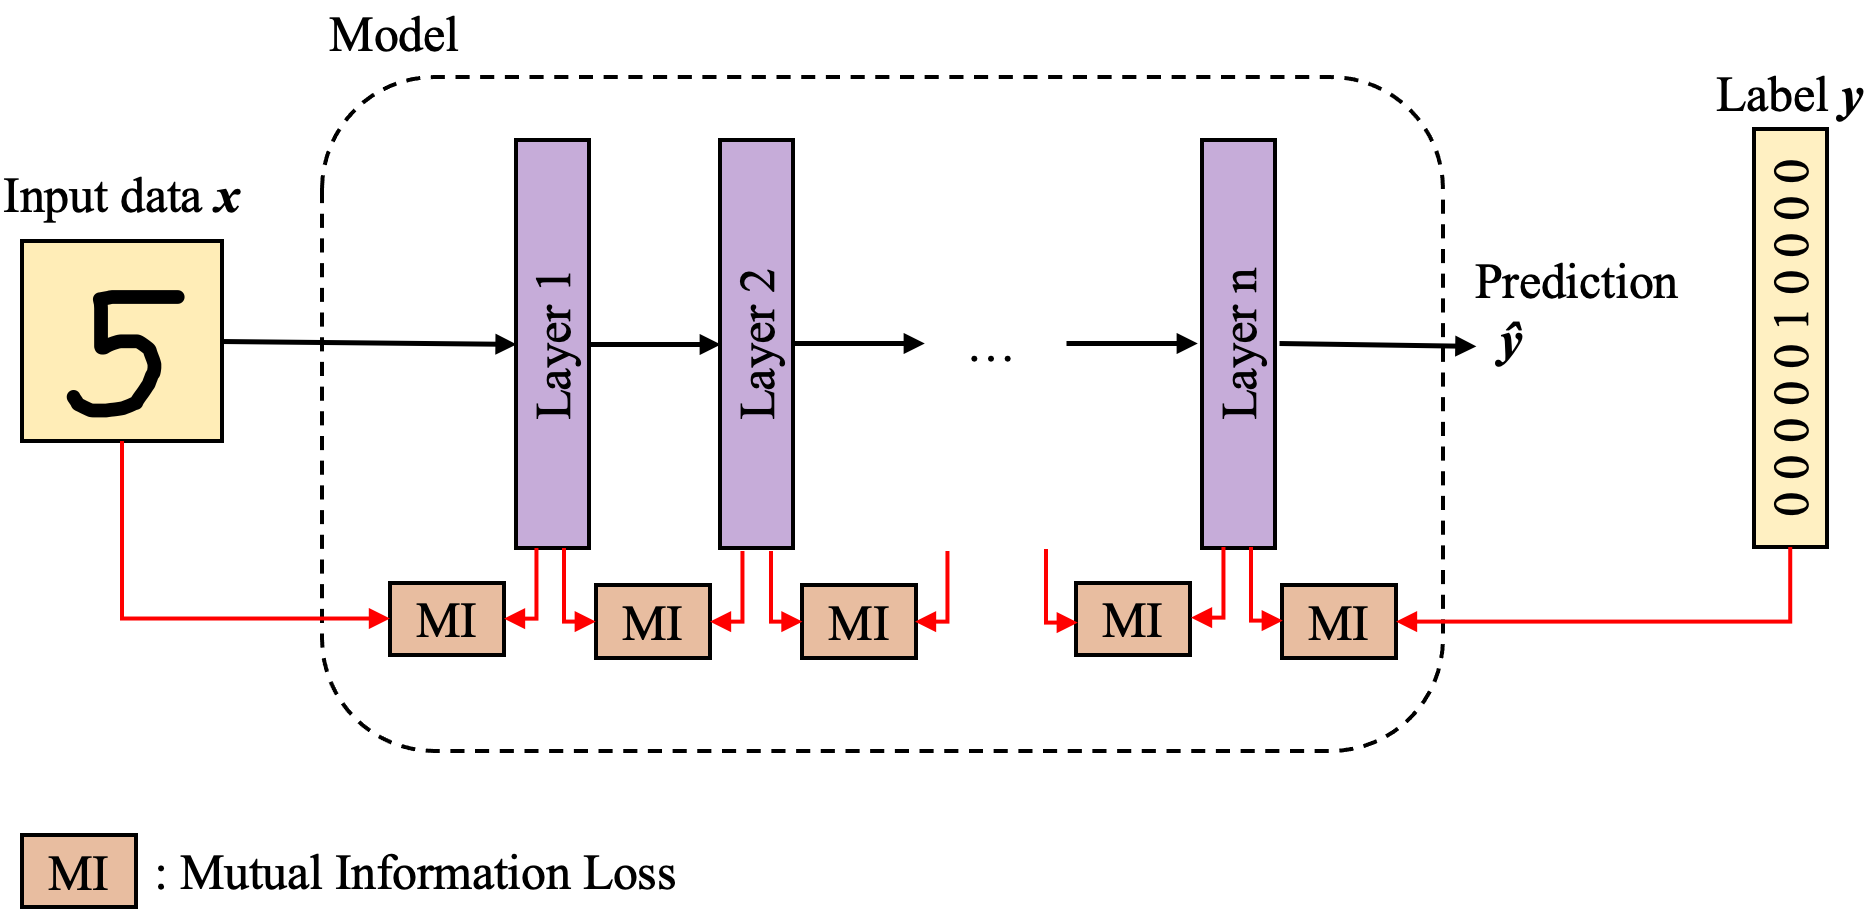
\includegraphics[width=0.99\textwidth]{mi_loss}
    \caption[Horizontal self-organisation with mutual information loss]{Horizontal self-organisation with mutual information loss: Each layer maximises the mutual information (MI) between its activations and the activations of the previous and subsequent layers. The first layer maximises the MI between its activations and the input image (instead of the previous layer), and the last layer maximises the MI between its activations and the image label (instead of the subsequent layer).}
    \figlbl{mi_loss}
\end{figure}

In the following, an alternative is proposed which does not have this disadvantage: Identical to the FF algorithm, the image is fed into the network's input layer for multiple timesteps. Conversely, the label is not fed directly into the output layer but is made available to the last layer within the loss function. Each layer maximises the mutual information (MI)\sidenote{or another metric to measure the similarity between activations} between its activations and the activations of the previous and subsequent layers. Thus, the first layer maximises the MI between the input image and its activations, and the last layer maximises the MI between its activations and a label vector. This creates a feature pyramid in which a smooth transition from concrete samples to abstract class labels is learned. During inference, each layer produces a class specific activation pattern, and the last layer directly predicts latent representations that can be assigned to a class. This process is visualised in \figref{mi_loss}.  However, the effectiveness of the proposed measures have to be evaluated in future work.


%\subsubsection{Convolutional Architecture}
%In a CNN, the field of view in the first layers is restricted by design but becomes larger in subsequent layers. Consequently, using a CNN architecture instead of a model based on fully connected layers alleviates the problem of non-hierarchical features.
%
%
%\begin{figure}[h]
%    \centering
%    \resizebox{0.99\textwidth}{!}
%{
%\begin{tikzpicture}
%\tikzstyle{connection}=[ultra thick,every node/.style={sloped,allow upside down},draw=\edgecolor,opacity=0.7]
%\tikzstyle{copyconnection}=[ultra thick,every node/.style={sloped,allow upside down},draw={rgb:blue,4;red,1;green,1;black,3},opacity=0.7]
%
%
%\node[canvas is zy plane at x=0] (input) at (0,0,0) {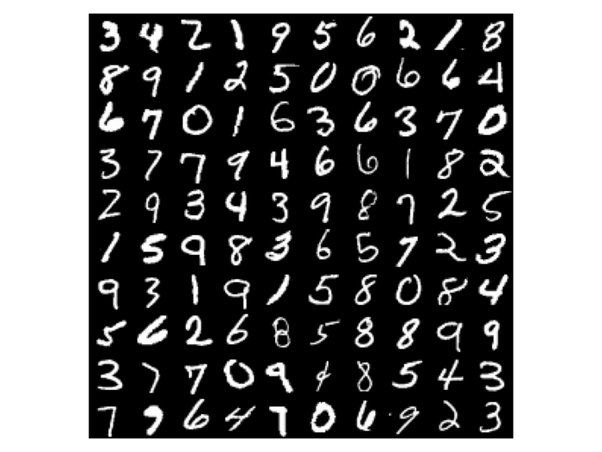
\includegraphics[width=8cm,height=8cm]{imgs/mnist.jpeg}};
%
%
%\pic[shift={(3,0,0)}] at (input) 
%    {Box={
%        name=conv1,
%        caption=Conv + ReLU,
%        xlabel={{1, }},
%        zlabel=16,
%        fill=\ConvColor,
%        height=16,
%        width=2,
%        depth=16
%        }
%    };
%
%
%\draw [connection]  (input) ++(0,0,0)    -- node {\midarrow} (conv1-west);
%
%
%\pic[shift={ (0,0,0) }] at (conv1-east) 
%    {Box={
%        name=pool1,
%        caption= ,
%        fill=\PoolColor,
%        opacity=0.5,
%        height=8,
%        width=1,
%        depth=8
%        }
%    };
%
%
%\pic[shift={(2,0,0)}] at (pool1-east) 
%    {Box={
%        name=conv2,
%        caption=Conv + ReLU,
%        xlabel={{16, }},
%        zlabel=32,
%        fill=\ConvColor,
%        height=8,
%        width=4,
%        depth=8
%        }
%    };
%
%
%\draw [connection]  (pool1-east)    -- node {\midarrow} (conv2-west);
%
%
%\pic[shift={ (0,0,0) }] at (conv2-east) 
%    {Box={
%        name=pool2,
%        caption= ,
%        fill=\PoolColor,
%        opacity=0.5,
%        height=4,
%        width=1,
%        depth=4
%        }
%    };
%
%
%\pic[shift={(2,0,0)}] at (pool2-east) 
%    {Box={
%        name=conv3,
%        caption=Conv + ReLU,
%        xlabel={{32, }},
%        zlabel=64,
%        fill=\ConvColor,
%        height=4,
%        width=6,
%        depth=4
%        }
%    };
%
%
%\draw [connection]  (pool2-east)    -- node {\midarrow} (conv3-west);
%
%
%\end{tikzpicture}
%}
%    \caption[Architecture of the CNN for horizontal self-organisation]{The network architecture of the CNN for horizontal self-organisation with fully connected layers.}
%    \figlbl{horizontal_org_arch2}
%\end{figure}
%
%The CNN architecture used in this thesis is shown in \figref{horizontal_org_arch2}.
%Three convolutional layers with ReLU activation functions and with $16$, $32$, and $64$ channels are used, and max-pooling layers are applied between each convolutional layer. For training, the same hyperparameters and loss functions are used for the model with fully connected layers.


%\subsubsection{Two-Way Information Flow}
%Hinton \sidecite{ff_algo} introduced with the forward-forward (FF) algorithm (c.f. \secref{alt_train_algo}) a promising idea for models based on proxy objective functions: 
%The image is fed into the input layer of the network, and the corresponding label is fed into the output layer of the network. The image remains static for several timesteps, and the network is trained to push the layer's activations above a certain threshold. In the second stage, the image is fed into the network with the wrong label and the network is trained to push the activations below a certain threshold. He found that a feature hierarchy is created when low-level features (i.e. images) are fed into the network from one end and high-level features (i.e. class labels) are fed into the network from the other end. However, this approach has one major disadvantage: During inference, each possible sample-label combination has to be fed into the model, and the label that caused the highest neural activity is used as the model's prediction.

%In this thesis, this process is implemented in a different way, which does not have this disadvantage. Identical to the FF algorithm, the image is fed into the network's input layer for multiple timesteps. Conversely, the label is not fed directly into the output layer but is made available to the last layer within the loss function. Each layer maximises the mutual information (MI) between its activations and the activations of the previous and subsequent layers. Thus, the first layer maximises the MI between the input image and its activations, and the last layer maximises the MI between its activations and a label vector. This creates a feature pyramid in which a smooth transition from concrete samples to abstract class labels is learned. During inference, the last layer directly predicts latent representations that can be assigned to a class. This process is visualised in \figref{mi_loss}. 

%\begin{figure}[h]
%    \centering
%    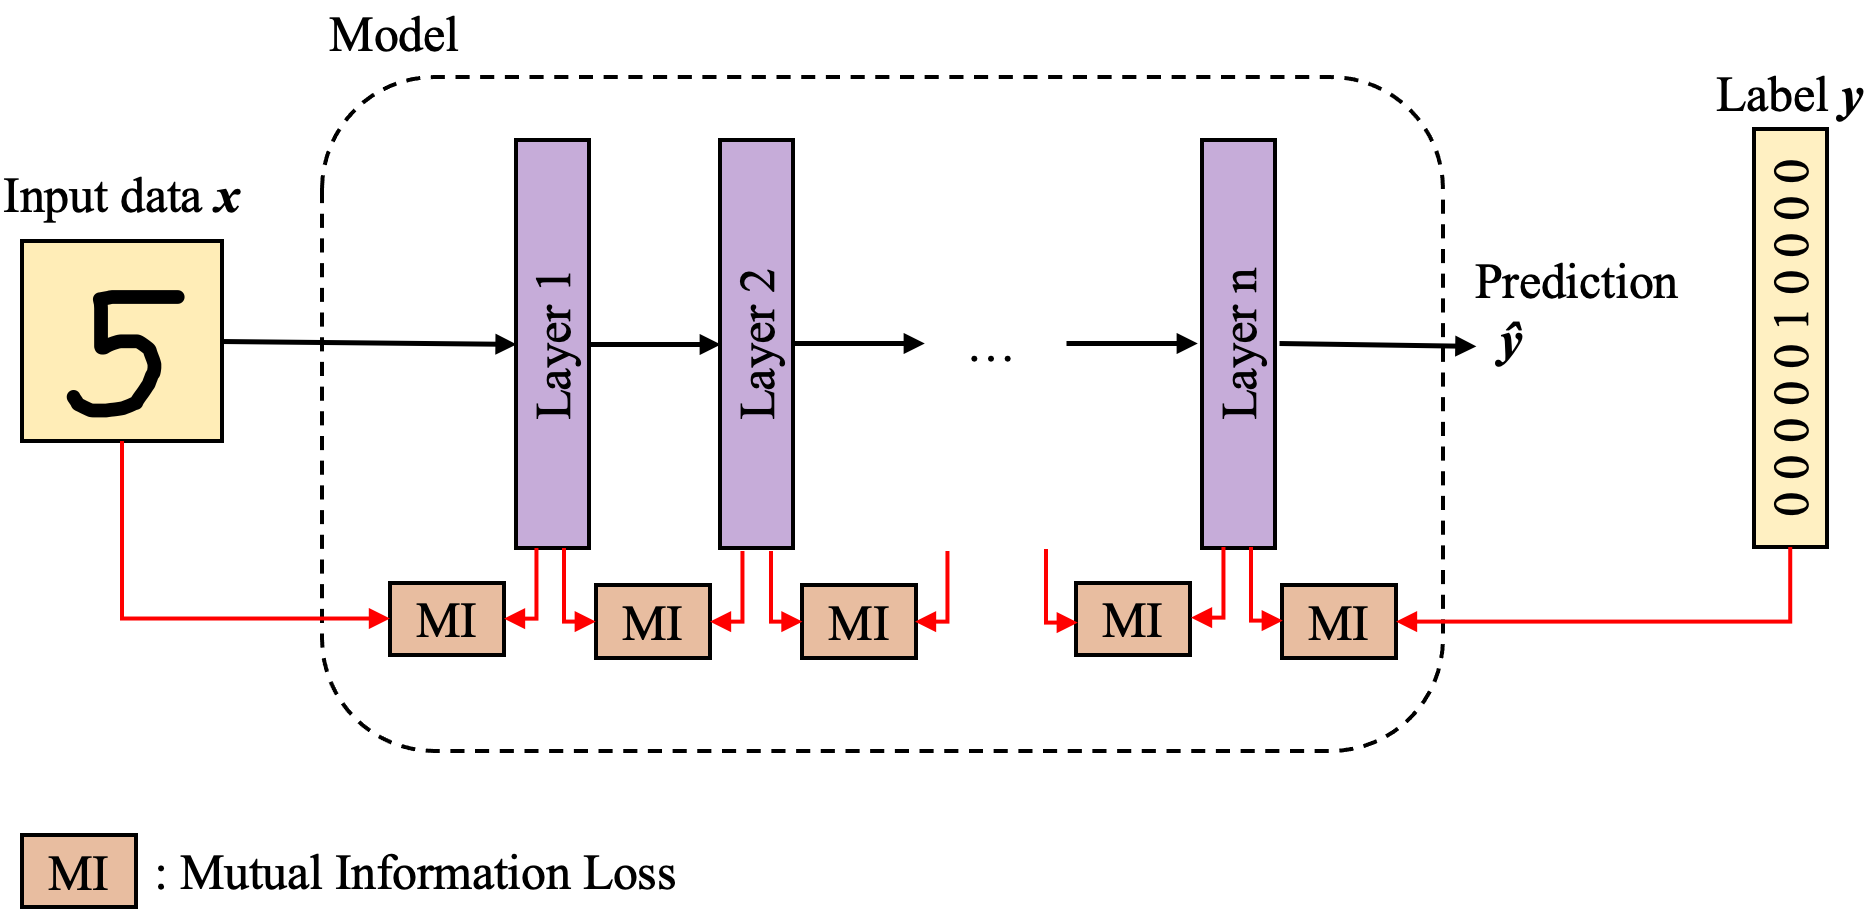
\includegraphics[width=0.99\textwidth]{mi_loss}
%    \caption[Horizontal self-organisation with mutual information loss]{Horizontal self-organisation with mutual information loss: Each layer maximises the mutual information (MI) between its activations and the activations of the previous and subsequent layers. The first layer maximises the MI between its activations and the input image (instead of the previous layer), and the last layer maximises the MI between its activations and the image label (instead of the subsequent layer).}
%    \figlbl{mi_loss}
%\end{figure}


\subsection{Vertical Self-Organisation}\seclbl{future_vso}
Vertical self-organisation splits the input image into multiple patches and processes the patches with independent models. Having multiple independent VAEs works worse than just having a single VAE that receives the entire image as input. However, by predicting larger output patches or adding lateral communication, the models without multiple VAEs create better lantent representations. This is demonstrated by the example of classification where an accuracy of up to $91.1\%$ is obtained on MNIST, significantly outperforming a single VAE that has an accuracy of $85.2\%$.
However, accuracy could be further improved: Currently, accuracy is calculated by comparing a sample with \emph{one} prototype per class. Using only one prototype might be not enough. For example, when looking at the t-SNE plots in \figref{hso_tSNE}, the same class is divided into more than one cluster. The calculation of the NMI score also indicates that one prototype per class is insufficient: When more clusters are used for k-means clustering, the NMI scores become higher. This is also in line with the findings of horizontal self-organisation (c.f. \secref{future_vso}) where using multiple prototypes significantly improved performance. Thus, the number of prototypes per class should be increased in future work.

An essential concept in the human brain is the prevention of early commitment \sidecite{Marr_2010} (c.f. \secref{future_3_stage}), i.e. that a single entity such as a network layer not commits to something and then persists. Typical CNN architectures for classification have this problem by design, as they combine low-level features into higher-level features. Low-level features are detected locally; thus, it is already determined which feature is within the image before global information is considered. The proposed architecture for vertical self-organisation reduces this problem by creating representations of image patches. The patches are so small that they contain only enough information to build low-level features. For example, the representations from a single VAE cannot be clearly assigned to a class and thus do not contain enough information to commit to higher-level features or an object. Therefore, the VAEs can be considered low-level feature extractors, such as the first layer of a convolutional network. To create higher-level features, communication with neighbouring VAEs (i.e. when looking at the big picture) is needed. Each VAE extracts low-level features (local view) and communicates with other VAEs (global view) to determine their representation. Therefore, this architecture is less susceptible to the early commitment problem than typical end-to-end trained neural networks.
Furthermore, the representations are learned unsupervised. For classification, the labels are fed into the network \emph{after} training in order to compute average class representations. Thus, no class representation but image compression is learned during training. This further reduces the problem of individual VAEs committing to a class.

However, future work should address a key problem of this architecture: Currently, this concept only works with images in which the objects always appear at approximately the same place in the image. This can be remedied if the VAEs are applied at different places in the image, similar to a kernel in a convolutional layer. In this case, however, the same VAE sees all image data, meaning that it implicitly receives local and global image information. This could reduce the independence of each VAE. Consequently, it should be investigated how this architecture can become translation invariant similar to CNNs.

Moreover, the communication between the VAEs is quite limited since only reconstructed data is forwarded. More sophisticated could be using a dedicated communication channel and letting the model decide on its own what kind of information is transmitted. One way to implement such a channel could be to add the communication data to additional channels: The input patch is fed into the first channel, and a reconstructed version is predicted in the first output channel. Thus, the first channel corresponds to a classic VAE. Additional channels in the input and output are used for communication. Therefore, each VAE not only outputs a reconstructed patch but also communication data that is added to the input data of its neighbouring VAEs. Thus, each VAE receives an input patch and input communication data and outputs the reconstructed patch and output communication data. 
The loss function remains the same for the first output channel since the goal is still the same, i.e. to reconstruct the output as well as possible and to have a well-shaped latent space. The only difference is that model can now access four input channels instead of one. However, the communication channels must be trained in order for them to be helpful for other VAEs. Therefore, an additional loss term mus be applied applied to the output communication channels. Since the VAEs are differentiable, one VAE can be trained by freezing the other VAEs and updating its weight in a way so that the performance of the other VAEs increases. Thereby, the output of the communication channels should improve in a way so that the other VAEs can benefit from it.




%\subsubsection{Communication Channel}
%Another way to communicate is through a dedicated communication channel. For this purpose, each VAE has not only $1$ input and $1$ output channel but $4$ input and output channels. The input patch is fed into the first channel, and a reconstructed version is predicted in the first output channel. Thus, the first channel corresponds to a classic VAE.
%The remaining three channels are for communication: Each VAE generates a separate communication output for its three neighbouring VAEs. Thus, each VAE receives an input patch to reconstruct and communicate data. These four input matrices are stacked and fed into the encoder. For example, the first VAE receives a given patch on the input channel $1$ and communication data from the 2nd, 3rd, and 4th VAE on the input channels $2$-$4$. Based on this information, it outputs a patch reconstruction on the output channel $1$ and communication data that is sent to the 2nd, 3rd, and 4th VAE on the output channels $2$-$4$. Thus, there is a dedicated two-way communication channel between each neighbouring VAE. This is shown in \figref{vae_comm_channel}.

%\begin{figure}[h]
%    \centering
%    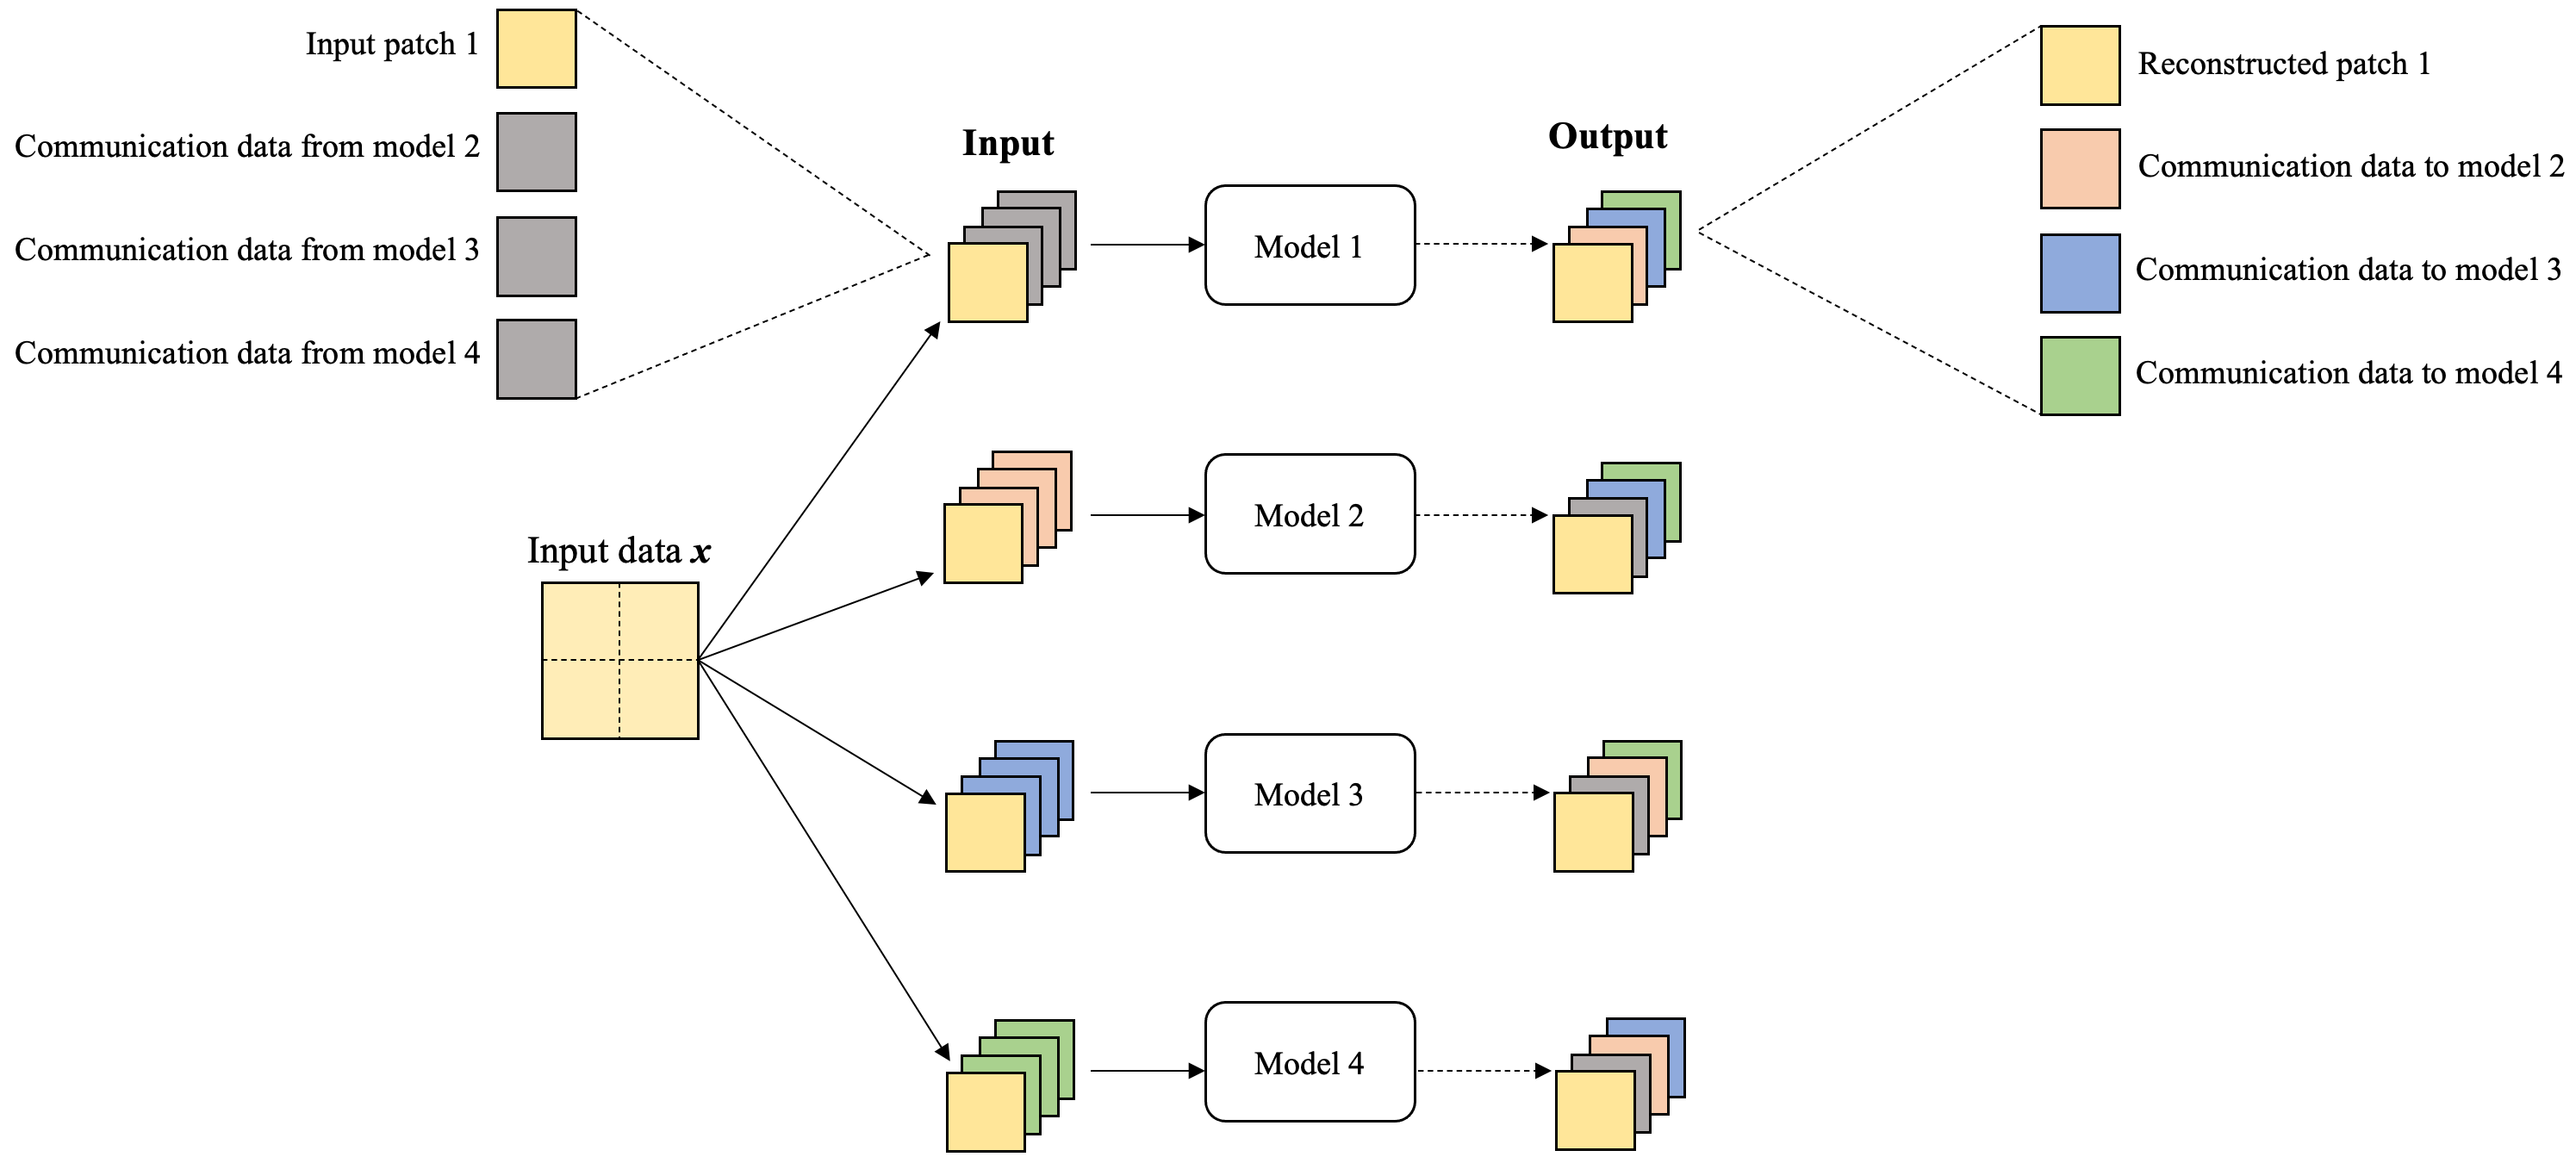
\includegraphics[width=0.89\textwidth]{vae_comm_channel}
%    \caption[Communication between VAEs with a dedicated communication channel]{Each VAE has one output channel to receive and reconstruct a given image patch. The other input and output channels are used for communication: Each VAE has for each other VAE a separate output channel to send messages and an additional input channel to receive messages.}
%    \figlbl{vae_comm_channel}
%\end{figure}

%The loss function remains the same for the first output channel since the goal is still the same, i.e. to reconstruct the output as well as possible and to have a well-shaped latent space. The only difference is that model can now access four input channels instead of one. However, the communication channels must be trained in order for them to be helpful for other VAEs. Therefore, an additional loss term is applied to the $3$ output communication channels. Thereby, the idea is to optimise the output of these communication channels so that the other VAEs can better reconstruct their patch.

%Let $V = \{V_1, ..., V_n \}$ be the set of $n$ VAEs. Each VAE has $n$ output channels, one channel for the reconstructed image and $n-1$ channels for communication. Furthermore, each VAE $V_i$ has a loss $\mathcal{L}_{\text{VAE}_i}$ based on the reconstruction goodness and the shape of the latent space (c.f. \eqref{hso_6}). The $3$ communication channels of VAE $i$ can influence the loss $\mathcal{L}_{VAE_j}$ of VAE $j$ (i.e. help to improve the loss by providing better information). How helpful the communication channels are can therefore be determined by the average loss of the other VAEs.

%\begin{align}\eqlbl{hso_9}
%	\mathcal{L}_{c_i} = \frac{1}{n-1} \sum_{n}^{j=1} \mathcal{L}_{\text{VAE}_j} \text{, if } i \neq j
%\end{align}

%Thus, the loss of a VAE with a communication channel is

%\begin{align}\eqlbl{hso_10}
%		\mathcal{L}_{{\text{VAE}_C}_i} = \mathcal{L}_{\text{VAE}_i} + \beta \cdot \mathcal{L}_{\text{KLD}_i} + \beta_2 \cdot \mathcal{L}_{c_i}
%\end{align}

%where $\beta_2$ is a weight factor for the communication channel. Thus, each model optimises its own reconstruction error, the shape of the latent space, and tries to improve the latent space and reconstruction error of other VAEs.



%\subsubsection{VQ-VAE}
%In the case of classification, the latent space has to be shaped in a way that allows to assign a latent representation to a class.
%This can be simplified if the encoder maps the input image to a discrete variable in the latent space.
%Vector quantised variational autoencoders (VQ-VAE) \sidecite{NIPS2017_7a98af17} model such a discrete latent space by using vector quantisation (VQ).
%Vector quantisation is a method that maps multi-dimensional vectors to a finite set of ``code''-vectors.
%Thus, an image is fed into the encoder to obtain the encoder output $\boldsymbol{h}_e$.
%Afterwards, a nearest neighbour lookup is made to find the code vector most similar to $\boldsymbol{h}_e$.
%The code-vector, also called the quantised vector $\boldsymbol{h}_q$, is fed into the decoder to reconstruct the image.



\section{3-Staged Model}\seclbl{future_3_stage}
TODO: Frame dieses Kapitel mehr so dass es klingt als wäre dies etwas on-top von VSO und HSO

Christoph von der Malsburg, co-supervisor of this thesis and one of the authors of the ``Theory of Natural Intelligence'' paper\sidenote{the work that served as \emph{the} source of inspiration of this thesis} \sidecite{von_der_Malsburg_Stadelmann_Grewe_2022}, is a pioneer of the theory of self-organising fibre connections in the visual system \sidecite{Wolfrum_Wolff_Lücke_vonderMalsburg_2008, Willshaw_VonDerMalsburg_1979, wiskott1996face, Fernandes_vonderMalsburg_2015}. His theory refers to an image perception model with three stages S$1$-S$3$, and projection fibres between these stages.
The stage S$1$ refers to the first stage, which is responsible for the extraction of features from images. In this stage, one fundamental principle is to avoid the ``fallacy of early commitment'' \sidecite{Marr_2010}.
The idea is that local decisions should only be taken if plausible in the light of high-level features, while high-level features can only be defined based on low-level patterns.
The brain can handle this very well, as the Gestalt psychology demonstrates\sidenote{Gestalt psychology is about intelligent beings perceiving entire patterns, not individual components} \sidecite{kohler1929gestalt}.
Convolutional networks, on the other hand, extract local low-level patterns in the first layers and compose them into higher-level patterns in subsequent layers. Thus, by definition, the first layers commit to a pattern based on local information without considering global information.

The $3$-staged model does not suffer from this problem: The stage S$1$ extracts local features. However, no commitment to higher-level features is made. Stage S$2$, on the other hand, contains object representations. The local features from S$1$ are mapped to S$2$ with bi-directional projection fibres. This mapping iteratively composes low-level features into high-level features. Thus, local information from S$1$ is used to find a suitable object representation in S$2$ and vice versa. These stages are described in more detail in the following.
Stage S$1$ is a mechanism based on lateral connections between neurons that are spatially close to each other. Initially, many neurons are activated by the retina's impulses. However, these neurons are immediately turned off if they do not have sufficient lateral support from neighbouring neurons. The lateral connections are thus used to keep each other active. This not only has the effect of ``mutually confirming each other'' but also helps to form higher-level features from low-level patterns: There are oscillations in the brain that also influence the number of active neurons. In other words, the number of active neurons continuously increases and decreases. Only those with enough local support remain if the number of active neurons is reduced. Thus, many neurons are deactivated in a short time. With each reduction of active neurons, higher-level features (so-called net fragments) are selected through lateral support.
Since only pixel groups that support each other remain active, neurons that represent insignificant features are continually switched off.

The lateral support, however, is limited to local patterns, i.e. the lateral support in S$1$ is not sufficient to recognise whole objects or scenes, but only parts of them. In stage S$2$, however, entire objects are represented. These object representations in S$2$ are independent of transformation and position. Projection fibres do the mapping of several low-level features in S$1$ to a concrete object in S$2$. These fibres implicitly remove transformations and position information from the features and assemble them into objects. Projection fibres can be interpreted as a kind of graph that combines features hierarchically, ignoring local distortions to create transformation-independent object detection. Stage S$3$, on the other hand, stores very abstract prototypes of such objects, and by matching S$2$ and S$3$, the captured object instances can finally be related to the brain's memory.

The $3$-staged model fundamentally differs from current CNN architectures and includes promising concepts such as preventing early commitment and using dynamic fibres. However, a concrete implementation that works for complex images like natural photos has yet to be implemented, despite a lot of effort in research. The model based on vertical self-organisation could be used as a feature extractor. This model is well suited because only local features are extracted that cannot be assigned to an object and thus have no early commitment. However, future work needs to extend this architecture with projection fibres.  %There is potential in using the recently popularised graph networks as projection fibres and thus learning the projections without relying on restricted mathematical models. For example, VAE or VQ-VAE, as in vertical self-organisation, could be used as feature extractors. The advantage of these autoencoder types is that they can extract local patterns and describe them as vectors in a ``meaningful'' latent space, i.e. similar vectors lie closer together in the latent space or, in the case of VQ-VAEs, are even discrete values. This facilitates the statistical learning and mapping of similar embedding vectors together. Vertical self-organisation (c.f. \secref{future_vso}) is considered an important preliminary work to implement such a system. In contrast to vertical self-organisation, autoencoders could be applied at any image position to obtain continuous pixel representations from the same latent space. The autoencoders can thus be used as feature extractors to extract good representations of small image patches. Afterwards, graph neural networks (GNNs) could be used to combine the embedding vectors into higher-level features. GNNs have already been used for image classification in recent years, mainly by identifying super-pixels and connecting them by graphs to recognise object structures \sidecite{Long_yan_chen_2021}.  One problem with GNNs is that they are often flat, i.e. many nodes lie on the same plane. This does not comply with the model of projection fibres, which must be highly hierarchical due to the large number of possible pattern combinations. A remedy to this issue could be using differential pooling \sidecite{10.5555/3327345.3327389, Vasudevan_Bassenne_Islam_Xing_2023}.

%However, the goal is not to identify objects with graph structures. Instead, the graph should be able to match objects from images with abstract prototypes. In this way, the network should learn to ignore slight transformations and rotations. For example, GNNs for object recognition could be combined with graph matching networks \sidecite{li2019graph, Xu_Nikolentzos_Vazirgiannis_Boström_2022} and thus might be used to match objects locally and globally despite slight transformations. This matching would correspond to projection fibres from L$1$ to L$2$ and compare objects within an image with mental prototypes. However, many questions remain, such as how objects are identified in images (i.e. how to remove the background) or how the mental prototypes get into L$2$ in advance in order that they can be matched. Furthermore, one must consider iterative matching to avoid early commitment: Low-level features should not commit to an object. Therefore, low-level features have to be extracted, and only a global view of all features allows to give them meaning. Thus, the learning process might iterate between updating features locally and giving them meaning in the global context.


\section{Useful Representations}\seclbl{useful_representations}
In this thesis, models are proposed that extract representations of images.
However, the question of how useful these representations are still remains\sidenote{despite the usual ML tasks such as image classifications}.

The usefulness of representation depends on the use case: Usually, good representations should contain exactly the information that is needed\sidenote{retaining as much information as possible is often not useful as this corresponds to storing (a compressed version) of the image} (i.e. be compact), be robust, be interpolatable, and be well-aligned with the real world.
For example, representations from modern deep learning systems are very useful for typical vision tasks such as classification or segmentation. In some cases, it could be argued that deep learning representations are even superior to humans: For example, modern deep learning systems \sidecite{DBLP:conf/bmvc/JungLO0SP22} can identify millions of faces with more than $99\%$ accuracy, which is very difficult for humans \sidenote{at least to distinguish such a large number of people}. 
However, what works poorly for deep learning systems is recognising an object as the same instance, regardless of which transformations have been applied. In general, deep learning systems cannot learn a good world model and understand transformations applied to various objects with different characteristics.

One way to address this problem is to allow the model to interact with the world (i.e. perform actions). Interacting allows a model to learn how an action changes the view of an object. Object-independent transformations such as rotations can be learned if the same actions are applied to different objects. This could allow a model to understand which views represent the same object in the world model and what kind of transformations have been applied to it.

It is known from the study of animals that both eye movements and the behavioural state influence the responses of neurons in the visual cortex \sidecite{Keller_Bonhoeffer_Hübener_2012}.
Thus, animals integrate their action (i.e., their movement) with currently incoming sensory signals to predict future sensory inputs.
The internal copy of an outflowing movement-producing signal generated by an organism's motor system is also known as efference copy.
Keurti et al. \sidecite{Keurti_Pan_Besserve_Grewe_Schölkopf_2022} argue that such efference copies are helpful to learn \emph{useful} latent representations perceived by the visual system.
They translated this idea into an AI-based system by allowing an agent to interact with the environment and observe its state to build internal representations.
They enforce that transformations of the real world can also be applied to latent representations, i.e. that the mental objects and the real-world objects remain consistent when similar transformations are applied to them.

Giving an agent an embodiment\sidenote{in this context, an embodiment can also be virtual, i.e. allow the agent to interact with objects} to interact with the world to better understand it and to create better representations seems not only important from a neuroscientific perspective but is also in line with theories from psychology.
Piaget \sidecite{Piaget_1964} argues that perceiving an object is rather about understanding how it transforms and behaves and not creating a mental copy of it.

Such an agent can be implemented, for example, with reinforcement learning.
The training process could be explicitly modelled by predicting future states based on a given state and possible actions before the action is executed and the actual outcome is observed in the world model.
This procedure corresponds to the perception-action episode that is postulated by LeCun \sidecite{LeCun_AMI}.
He divides the process into seven steps;
(i) First, the perception system extracts a representation of the current state of the world $s[0]=P(x)$. (ii) The actor then proposes an initial sequence of actions $(a[0], ..., a[t], ... a[T])$ that the virtual world model executes. (iii) The world model, in turn, predicts a sequence of world state representations resulting from the proposed action sequence $(s[1], ..., s[t], ... s[T])$. (iv) A cost model estimates the total costs for each state sequence as a sum over time steps $F(x)=\sum_{t=1}^{T}C(s[t])$. (v) Based on multiple cost predictions, the actor proposes the action sequence with the lowest costs. (vi) The actor executes one or a few actions (and not the entire action sequence), and the entire process is repeated. (vii) Additionally, every action, the states and associated costs are stored in a short-term memory that can be used to optimise the system.

Overall, it seems very important that a model does not receive a sequence of unrelated images and their labels as input, as in typical classification tasks. Instead, the agent should receive a continuous stream of related input images and information about their transformation. In this way, transformations can be observed and learned, which is fundamental to understanding visual scenes.

\section{Cognition and Reasoning}\seclbl{cognition_reasoning}
At the end of this thesis, I want to share my personal opinion on how deep learning systems can be improved fundamentally: Deep learning systems can extract pixel representations from images very well. I intentionally call it ``pixel''-representations and not object representations because these vectors contain information about pixel constellations which are not sufficient to describe objects but very well suited for tasks like classification or segmentation\sidenote{end-to-end backpropagation of error seems to work excellent to generate ``pixel''-representations}. According to my definition, these pixel representations are only a part of object representations. Object representations are mental constructs that contain much more information about objects than how they look. For example, object representations should contain information about how an object behaves under different transformations. In the previous two sections (c.f. \secref{future_3_stage}, \secref{useful_representations}), it is discussed how such transformations could be learned. However, many other parameters make up an object, such as its abilities (e.g. can it move?) and how it feels. The appearance of an object (which corresponds to the pixel representations) is thus only one dimension of a high-dimensional formula that describes an object. For example, fish and ships look completely different on a pixel-level description and have visually nothing in common. However, for us humans, these two objects have a clear relationship defined by their ability to swim and the typical place where they are found, i.e. the sea. Another example is heat: It feels hot, and in my mental world model have things like fire, the blue flame of a welding machine, and a hob, an obvious relationship. However, all these objects look completely different.
Many modern pattern extraction systems only model one-dimensional pixel representations and not multi-dimensional object representations and thus cannot build such relationships.
Extending these one-dimensional object representations (``what does the object look like'') to multi-dimensional representations might be one of the key elements to creating a system with cognition and reasoning. This allows object hierarchies to be built on multiple dimensions: Instead of just a hierarchy of objects that look similar, we also need hierarchies of objects that behave similarly, have similar capabilities, feel similar, etc.

In addition to this construction of multi-dimensional object representations, an understanding of the world's physics is necessary. This second type of representation summarises knowledge that relates to all objects, for example, the earth's gravitational force, the fact that living beings cannot walk through solid materials such as walls, etc. The question that arises now is how such a system can be implemented. It is obvious that more than simply showing pictures and the corresponding labels is required to learn such complex relationships. At least three key elements are required:


\begin{description}
	\item[The world] in which the agent lives must allow interactions. This allows the agent to learn representations better; for example, getting visual observations together with efference copies allows an agent to understand how objects behave. Furthermore, such a world allows understanding differences and similarities between objects. It also allows the agent to define what it does not yet know and to learn these things consciously (for example, with an entropy-based loss function \sidecite{storck1995reinforcement}). Thus, also continuous input is necessary. Training a model with a sequence of random and unrelated images is most likely not sufficient.
	\item[The network architecture] must enable and encourage the capture of the world's structure. I think that a mental multi-dimensional world model is helpful for storing and relating the appearance, behaviour, transformation capabilities, abilities, etc., of each object and a second model to store general knowledge about the world. Such an architecture allows modelling a multi-dimensional relationship between objects\sidenote{in a purely visual perception model, a division into the dimensions of appearance, behaviour during transformation, and physics (e.g. the object is standing on the ground) would already be a massive step forward}.% Multi dimensional world model, per object appearance, transformation behaviour, abilities, feeling, smell, ...
	\item[The learning algorithm] should consider several things to learn a good world model: A key element is that the learning algorithm decides what to learn (entropy based on the knowledge in the world model). Furthermore, curriculum learning seems promising: For a high level of intelligence, an equally complex world must be available in order to be able to learn it. However, such worlds might be so complex that the agent is overwhelmed without a step-by-step complexation of the world\sidenote{this also applies to humans: We need prior knowledge to survive - We have prior knowledge through evolution, and, after birth, our parents explain the world to us. In fact, we are not able to survive without proper support in the first years}.% continuous learning, curriculum learning % LLM -> predicten next token -> predicten objects next state
\end{description}

An intelligent system consists of several components: One very crucial component is the perception system. From today's point of view, this is the component that is best mastered, i.e. deep learning systems can capture useful patterns in high-dimensional data very well\sidenote{although there are things that need to be improved, c.f. \secref{future_3_stage}}. Around this system, a world model has to be created, which stores the understanding of the world. It is important that the agent learns to learn, i.e. finds out for itself what knowledge it lacks in the world model and acquires it from the real world. Such behaviour can be implemented by an entropy-based loss function \sidecite{storck1995reinforcement}. The second question is what knowledge is extracted from the world and stored in the world model (and thus implicitly defines what the agent learns). The knowledge stored in the world model should be multi-dimensional object information, as described in the first paragraph of this section, which provides a much richer understanding of the world than the current one-dimensional pixel representations. To get a real understanding of the world, interactions with the world and predictions of how the next state of the world looks seem to be very central\sidenote{for example, the simple task of predicting the next token of a text has led to the enormous capabilities of large language models}. A straightforward implementation is a roll-out (i.e. predict how the world looks like after applying some actions and comparing this to the real world after these actions have been applied) \sidecite{LeCun_AMI}, more advanced are GFlowNetworks \sidecite{NEURIPS2021_e614f646}. After such predictions are learned, reversing this process, as in diffusion models, could be a first step towards casual reasoning: In diffusion models, one learns to map from a specific state (a concrete image) to a very general state (noise). This process is reversed, and over several steps, the model can build trajectories from noise to a sample through a combination of direct and random motions. If a similar concept is applied to the learned prediction of actions, it can be predicted which action combinations have led to the current world state. However, all these ideas are very abstract and have emerged in the course of this work. The concretisation of these ideas could take years and, unfortunately, are out-of-scope of this thesis. However, I hope to be able to address such questions as concrete research topics soon, ideally in a similar constellation as in this Master's thesis.


